\section{Metodologia de Estimação da Temperatura Interna das Células}

\subsection{Introdução}
A monitoração da temperatura das células em um acumulador de alto desempenho (FSAE) é crítica não apenas para a segurança (evitar \textit{thermal runaway}), mas também para a otimização da entrega de potência. Sensores NTC convencionais, posicionados nos terminais ou na superfície das células, apresentam uma inércia térmica significativa e não capturam a temperatura real do \textit{jelly roll} (núcleo eletroquímico) durante transientes de alta corrente. Para mitigar esse atraso, a equipe implementou um \textbf{Estimador de Temperatura Interna baseado em Resistência de Pulso ($R_{dc}$)}, fundamentado no trabalho de Ludwig et al. (2022).

\subsection{Fundamentação Teórica}
A resistência interna de uma célula de Li-ion é fortemente dependente da temperatura, seguindo um comportamento descrito pela \textbf{Equação de Arrhenius}. Esse fenômeno ocorre porque a mobilidade iônica no eletrólito e a cinética de transferência de carga nos eletrodos são processos ativados termicamente.

O modelo adotado separa a resistência total da célula em uma componente ôhmica constante ($R_0$) e uma componente dependente da temperatura:

\begin{equation}
R_{dc}(T) = R_0 + R_1 \cdot e^{\left(\frac{E_a}{k_B T}\right)}
\end{equation}

Onde:
\begin{itemize}
    \item $R_{dc}$: Resistência interna total medida em DC.
    \item $R_0$: Resistência ôhmica fixa (contatos, abas, coletores).
    \item $R_1$: Fator pré-exponencial calibrado.
    \item $E_a$: Energia de ativação eletroquímica (eV).
    \item $k_B$: Constante de Boltzmann ($8.617 \times 10^{-5} eV/K$).
    \item $T$: Temperatura absoluta (Kelvin).
\end{itemize}

A Figura \ref{fig:arrhenius} apresenta a curva de caracterização para as células \textbf{Molicel P28A} utilizadas no projeto, demonstrando a sensibilidade da resistência interna em relação à temperatura.

\begin{figure}[H]
    \centering
    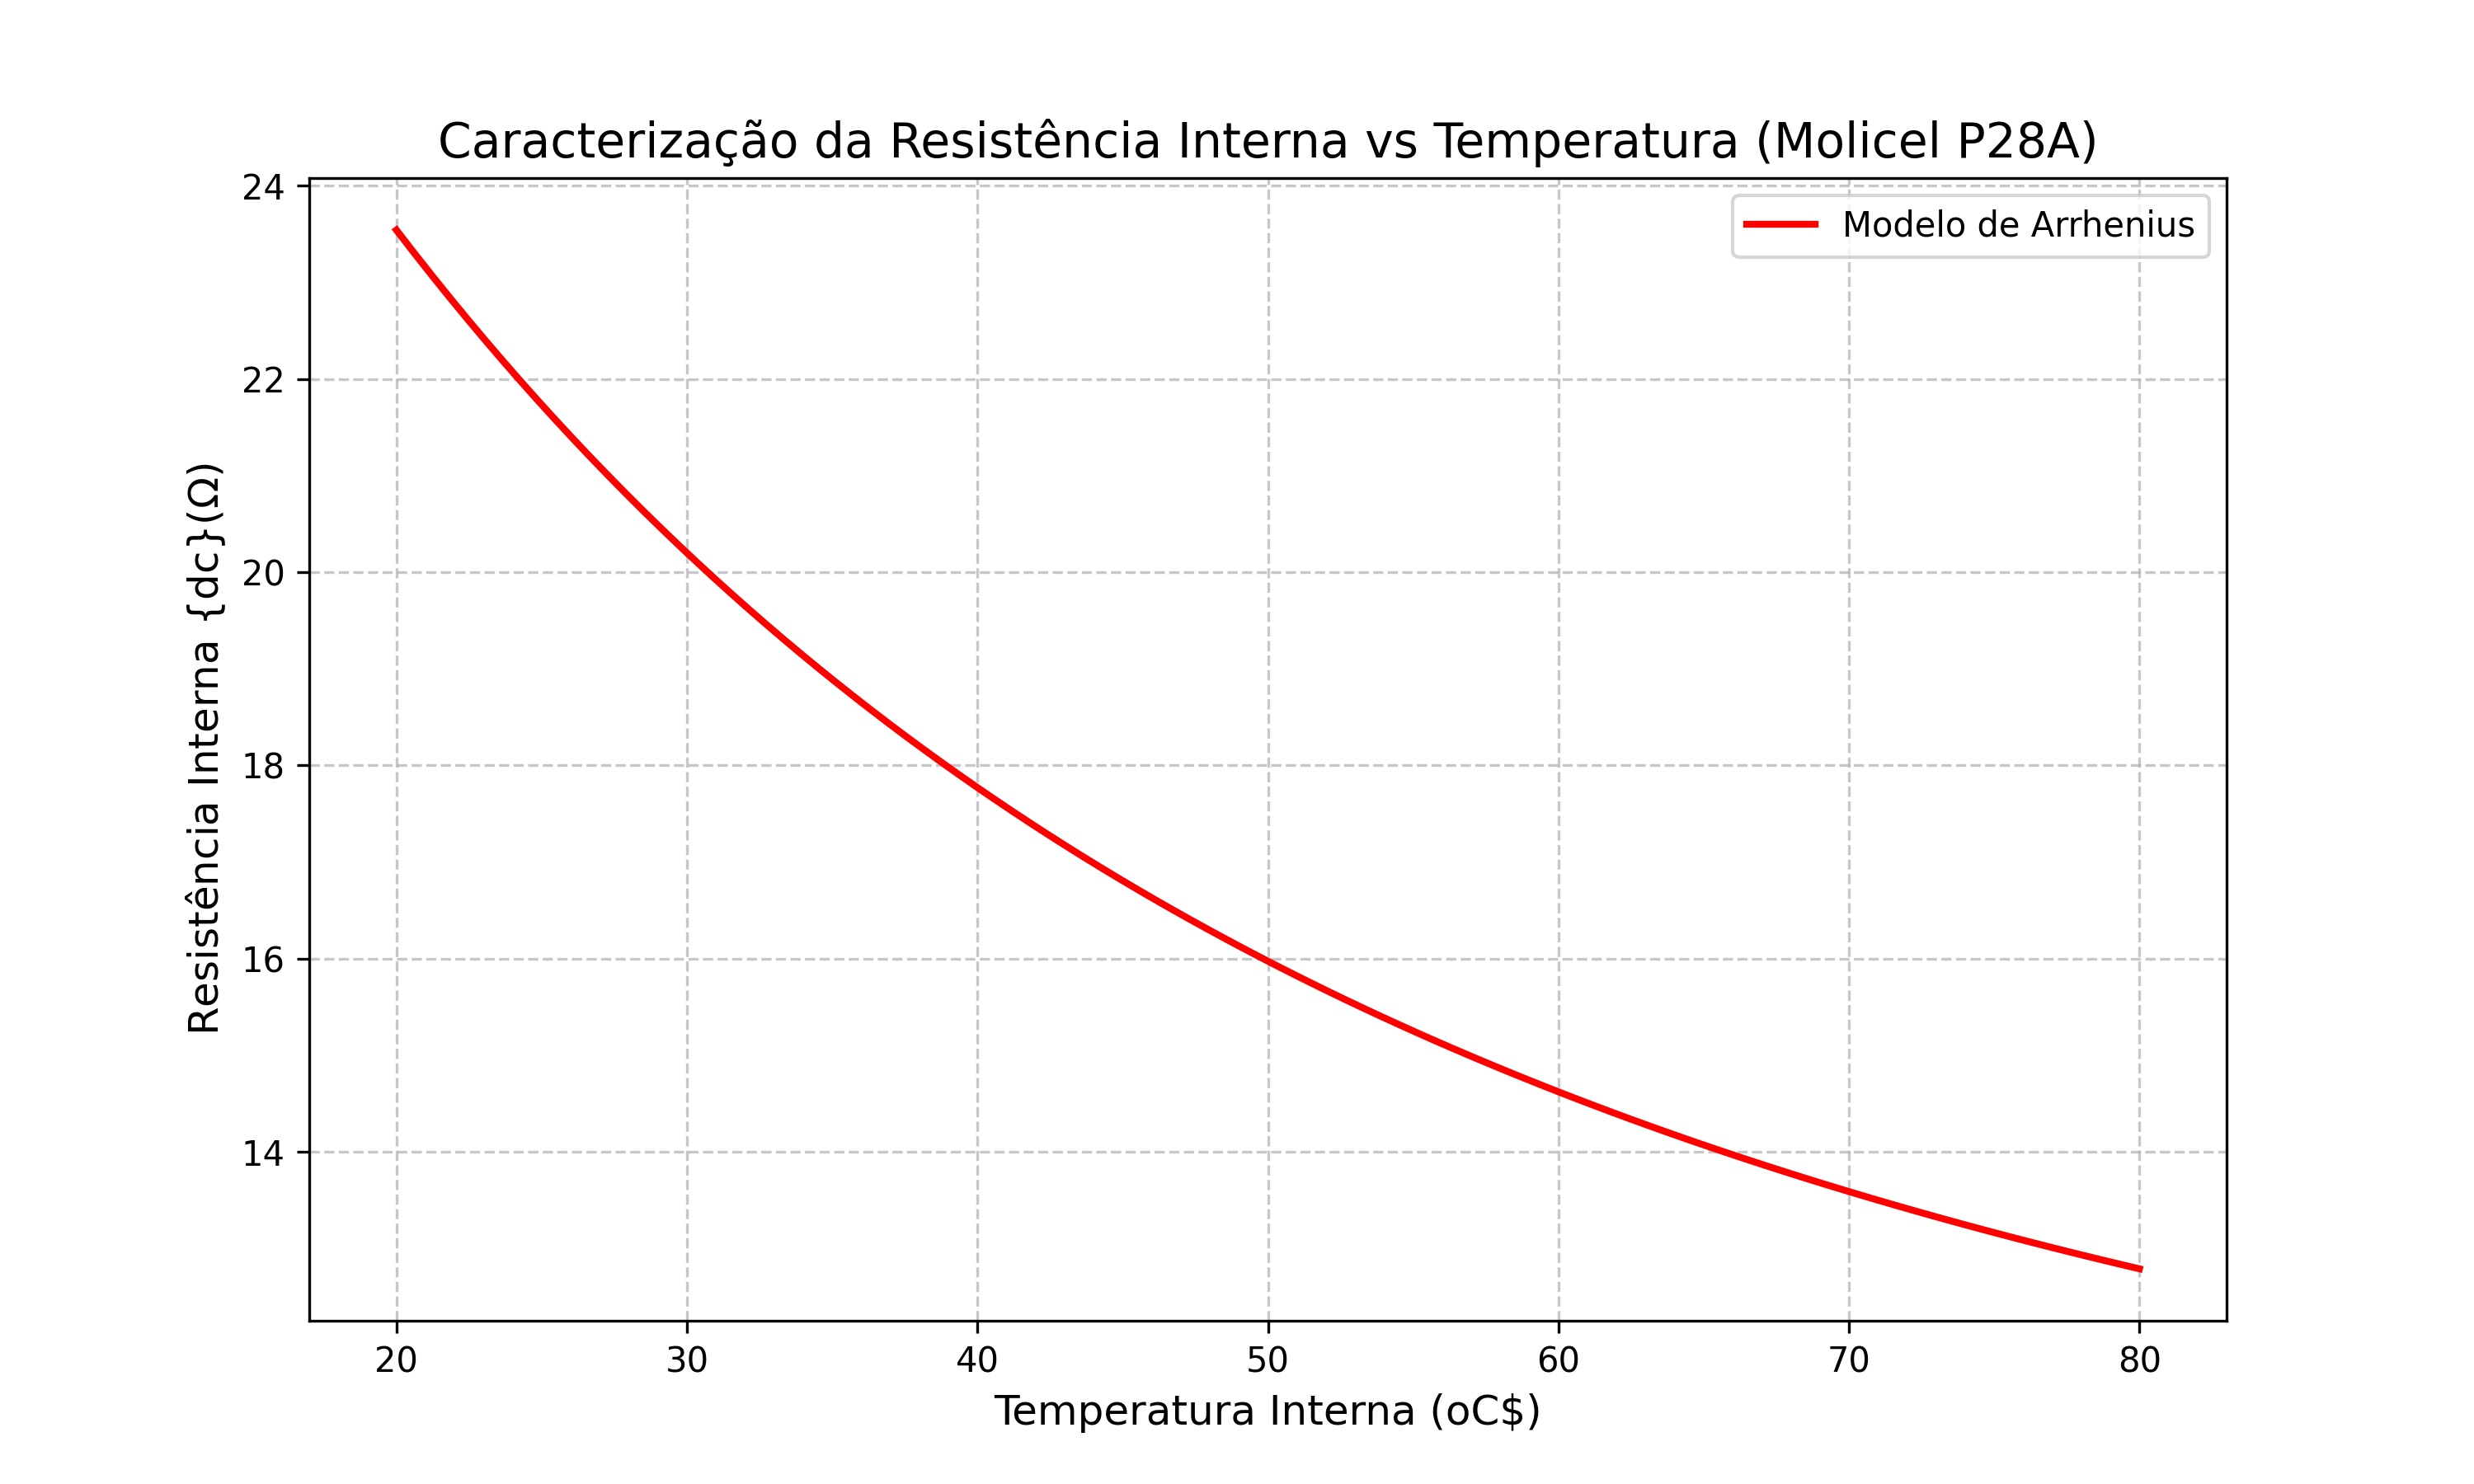
\includegraphics[width=0.8\textwidth]{arrhenius_curve.png}
    \caption{Curva de resistência interna vs temperatura baseada no modelo de Arrhenius.}
    \label{fig:arrhenius}
\end{figure}

\subsection{Implementação Prática e Detalhamento dos Passos}
O algoritmo foi implementado como uma máquina de estados síncrona que opera na frequência de amostragem do barramento CAN (tipicamente 100Hz na TMS Master). O processo é dividido em seis etapas fundamentais:

\subsubsection{Passo 1: Monitoramento de Repouso e Gatilho (Trigger)}
O sistema monitora continuamente a corrente ($I$) e a tensão ($V$). Enquanto a variação de corrente for inferior a $\Delta I_{threshold} = 2A$, o estimador permanece em estado de \textit{Idle}, atualizando apenas as ``estacas de ancoragem'' ($V_{pre}, I_{pre}$). Quando um degrau de corrente superior a $2A$ é detectado (ex: aceleração do piloto), o estado muda para \textit{Pulse Active} e um temporizador é iniciado.

\subsubsection{Passo 2: Janelamento Temporal (Settling Time)}
Diferente de uma leitura instantânea, o algoritmo aguarda $t_{wait} = 150ms$. Este atraso é crucial para garantir que as capacitâncias de dupla camada e os efeitos de difusão de curto prazo do Modelo de Circuito Equivalente (ECM) se estabilizem. Sem este janelamento, a resistência medida seria a resistência de transferência de carga momentânea, que não reflete fielmente a dependência térmica de Arrhenius do eletrólito e do \textit{jelly roll}.

\subsubsection{Passo 3: Extração Diferencial da Resistência ($R_{dc}$)}
Após os 150ms, uma nova amostra ($V_{now}, I_{now}$) é capturada. A resistência interna DC é calculada pela razão das variações:
\begin{equation}
R_{dc} = \frac{|V_{now} - V_{pre}|}{|I_{now} - I_{pre}|}
\end{equation}
Nesta etapa, o firmware aplica uma trava de segurança física: valores fora da faixa de $5m\Omega$ a $100m\Omega$ são descartados como ruído ou erro de amostragem, evitando que falhas de sensor corrompam a estimativa térmica.

\subsubsection{Passo 4: Seleção de Parâmetros por Estado de Carga (SOC)}
Como a energia de ativação ($E_a$) e o fator pré-exponencial ($R_1$) variam com a concentração de íons de lítio nos eletrodos, o algoritmo utiliza o SOC atual para indexar Tabelas de Pesquisa (LUTs). O SOC é dividido em 11 pontos (0\% a 100\%), e o firmware seleciona o conjunto de parâmetros ($R_0, R_1, E_a$) calibrados para a Molicel P28A naquele nível de carga específico.

\subsubsection{Passo 5: Cálculo da Temperatura Inversa}
Com os parâmetros e o $R_{dc}$ em mãos, aplica-se a função inversa de Arrhenius para isolar a temperatura absoluta ($T$):
\begin{equation}
T [K] = \frac{E_a}{k_B \cdot \ln\left(\frac{R_{dc} - R_0}{R_1}\right)}
\end{equation}
O resultado é então convertido para graus Celsius: $T [^{\circ}C] = T [K] - 273,15$.

\subsubsection{Passo 6: Filtragem e Saturação}
Devido ao achatamento da curva de Arrhenius em temperaturas elevadas (perda de sensibilidade do $R_{dc}$), amostras individuais podem apresentar ruído. O sistema utiliza um \textbf{Filtro de Média Móvel de 8 amostras}. Além disso, qualquer estimativa abaixo de $-20^{\circ}C$ ou acima de $100^{\circ}C$ é sumariamente descartada para evitar alarmes falsos em falhas de inicialização.

\subsection{Conclusão}
A integração deste modelo permite que o BMS antecipe o aquecimento interno das células muito antes dos sensores superficiais detectarem a variação. Isso possibilita uma estratégia de gerenciamento térmico mais agressiva e segura, protegendo a integridade química das células Molicel P28A durante as provas de Endurance.

\subsection{Referências}
\begin{enumerate}
    \item LUDWIG, S.; STEINHARDT, M.; JOSSEN, A. \textit{Determination of Internal Temperature Differences for Various Cylindrical Lithium-Ion Batteries Using a Pulse Resistance Approach}. MDPI Batteries, 2022, 8(7), 60.
    \item SCHMIDT, J. P. et al. \textit{The relation between the internal temperature of lithium-ion batteries and their ohmic resistance}. Journal of Power Sources, 2015, v. 287, p. 34-41.
    \item LUDWIG, S. et al. \textit{Influence of aging on the internal temperature estimation of lithium-ion batteries by resistance measurements}. Journal of Power Sources, 2022.
    \item MOLICEL. \textit{INR-21700-P28A Data Sheet}.
\end{enumerate}
